\documentclass[aspectratio=169, 10pt]{beamer}

\usetheme{metropolis}
\usetikzlibrary{shapes, snakes, spy, positioning}

\setbeamercolor{background canvas}{bg=white}

\metroset{
  numbering=fraction,
  progressbar=frametitle,
  block=fill,
}

\usefonttheme[onlymath]{serif}

\usepackage[ngerman]{babel}
\usepackage[style=iso-numeric]{biblatex}
\usepackage{csquotes}
\usepackage{mathtools, graphicx, booktabs, pgfplots, xcolor}
\usepackage[font=footnotesize]{caption}
\usepackage{listings}
\usepackage{hyperref}

\definecolor{mDarkBrown}{HTML}{604c38}
\definecolor{mDarkTeal}{HTML}{23373b}
\definecolor{mLightBrown}{HTML}{EB811B}
\definecolor{mLightGreen}{HTML}{14B03D}
\definecolor{mBackground}{HTML}{FFFFFF}
\definecolor{myblue}{HTML}{6699cc}
\definecolor{myorange}{HTML}{eb801a}

\lstset{%
  language=Python,
  basicstyle=\small\ttfamily,
  keywordstyle=\color{mLightBrown}\bfseries,
  commentstyle=\color{mLightGreen},
  stringstyle=\color{mLightGreen},
  backgroundcolor=\color{mBackground},
  numbers=none,
  numberstyle=\tiny\ttfamily,
  stepnumber=2,
  showspaces=false,
  showstringspaces=false,
  showtabs=false,
  frame=none,
  framerule=1pt,
  tabsize=2,
  rulesep=5em,
  captionpos=b,
  breaklines=true,
  breakatwhitespace=false,
  framexleftmargin=0em,
  framexrightmargin=0em,
  xleftmargin=0em,
  xrightmargin=0em,
  aboveskip=1em,
  belowskip=1em,
  morekeywords={usetheme,institute,maketitle,@metropolis@titleformat,%
                plain,setbeamercolor,metroset,setsansfont,setmonofont},
}


\addbibresource{bibliography.bib}
\graphicspath{{./Grafiken/}}
\captionsetup{belowskip=0pt}

\newcommand{\dnn}[1]{
  \def\layersep{2.5cm}
  \def\list{#1}
  \begin{tikzpicture}[->, >=stealth, node distance=\layersep]
    \tikzstyle{every pin edge}=[<-,shorten <=1pt]
    \tikzstyle{neuron}=[circle,draw,minimum size=17pt,inner sep=0pt]
    \pgfmathsetmacro{\numl}{dim({\list})}
    \pgfmathsetmacro{\numh}{\numl-1}
    \pgfmathsetmacro{\numi}{{\list}[0]}
    \pgfmathsetmacro{\numo}{{\list}[\numl-1]}

    % Draw the input layer
    \foreach \y in {1,...,\numi}
    \node[neuron, pin=left:\(x_{\y}\)] (I-\y) at (0,-\y) {};

    % Draw the hidden layers
    \foreach \y [count=\i, evaluate=\i as \break using \i + 2] in \list {
      \pgfmathsetmacro{\counti}{{\list}[\i]}
      \foreach \x in {1,...,\counti} {
        \path[yshift=(\counti cm - \numi cm)/2] node[neuron] (H\i-\x) at (\i * \layersep, -\x cm) {};
      }
      \ifnum \numl=\break
      \breakforeach
      \fi
    }

    % Draw the output layer nodes
    \foreach \y in {1,...,\numo}
    \path[yshift=(\numo cm - \numi cm)/2] node[neuron,pin={[pin edge={->}]right:\(y_{\y}\)}] (O-\y)  at (\numh * \layersep, -\y cm) {};

    % Connect Input layer and first hidden layer
    \pgfmathsetmacro{\lhonenum}{{\list}[1]}
    \foreach \source in {1,...,\numi}
    \foreach \dest in {1,...,\lhonenum}
    \path (I-\source) edge (H1-\dest);

    \foreach \y [count=\i, evaluate=\i as \break using \i + 3] in \list {
      \pgfmathsetmacro{\curr}{int({\list}[\i])}
      \pgfmathsetmacro{\next}{int({\list}[\i+1])}
      \pgfmathsetmacro{\j}{int(\i+1)}
      \foreach \source in {1,...,\curr}
      \foreach \dest in {1,...,\next}
      \path (H\i-\source) edge (H\j-\dest);
      \ifnum \numl=\break
      \breakforeach
      \fi
    }

    % Connect last hidden layer with output layer
    \pgfmathsetmacro{\lmone}{{\list}[\numl-2]}
    \pgfmathsetmacro{\lmonenum}{int(dim({\list})-2)}
    \foreach \source in {1,...,\lmone}
    \foreach \dest in {1,...,\numo}
    \path (H\lmonenum-\source) edge (O-\dest);
    \node[node distance=1.9cm, above of=H2-1] (hidden) {Hidden Layers};
    \node[node distance=2*\layersep, left of=hidden] {Input Layer};
    \node[node distance=2*\layersep, right of=hidden] {Output Layer};
    \draw[-, decorate, decoration=brace, thick] (2.1cm, .5cm) -- (7.8cm, .5cm);
  \end{tikzpicture}
}

%%% Local Variables:
%%% mode: latex
%%% TeX-master: "../präsentation"
%%% End:


\title{Algorithmik zur Optimierung in neuronalen Netzwerken}
\subtitle{Gradient Descent und Backpropagation}
\institute{Hochschule Esslingen --- University of Applied Sciences}
\author{Tim Hilt}
\date{19. Mai 2020}

\begin{document}

\begin{frame}
  \maketitle
\end{frame}

\begin{frame}{Gliederung}
  \tableofcontents
\end{frame}

\section{Supervised Learning}%
\label{sec:supervised}

\begin{frame}{Machine Learning Workflow}
  \begin{figure}[!htbp]
    \centering
    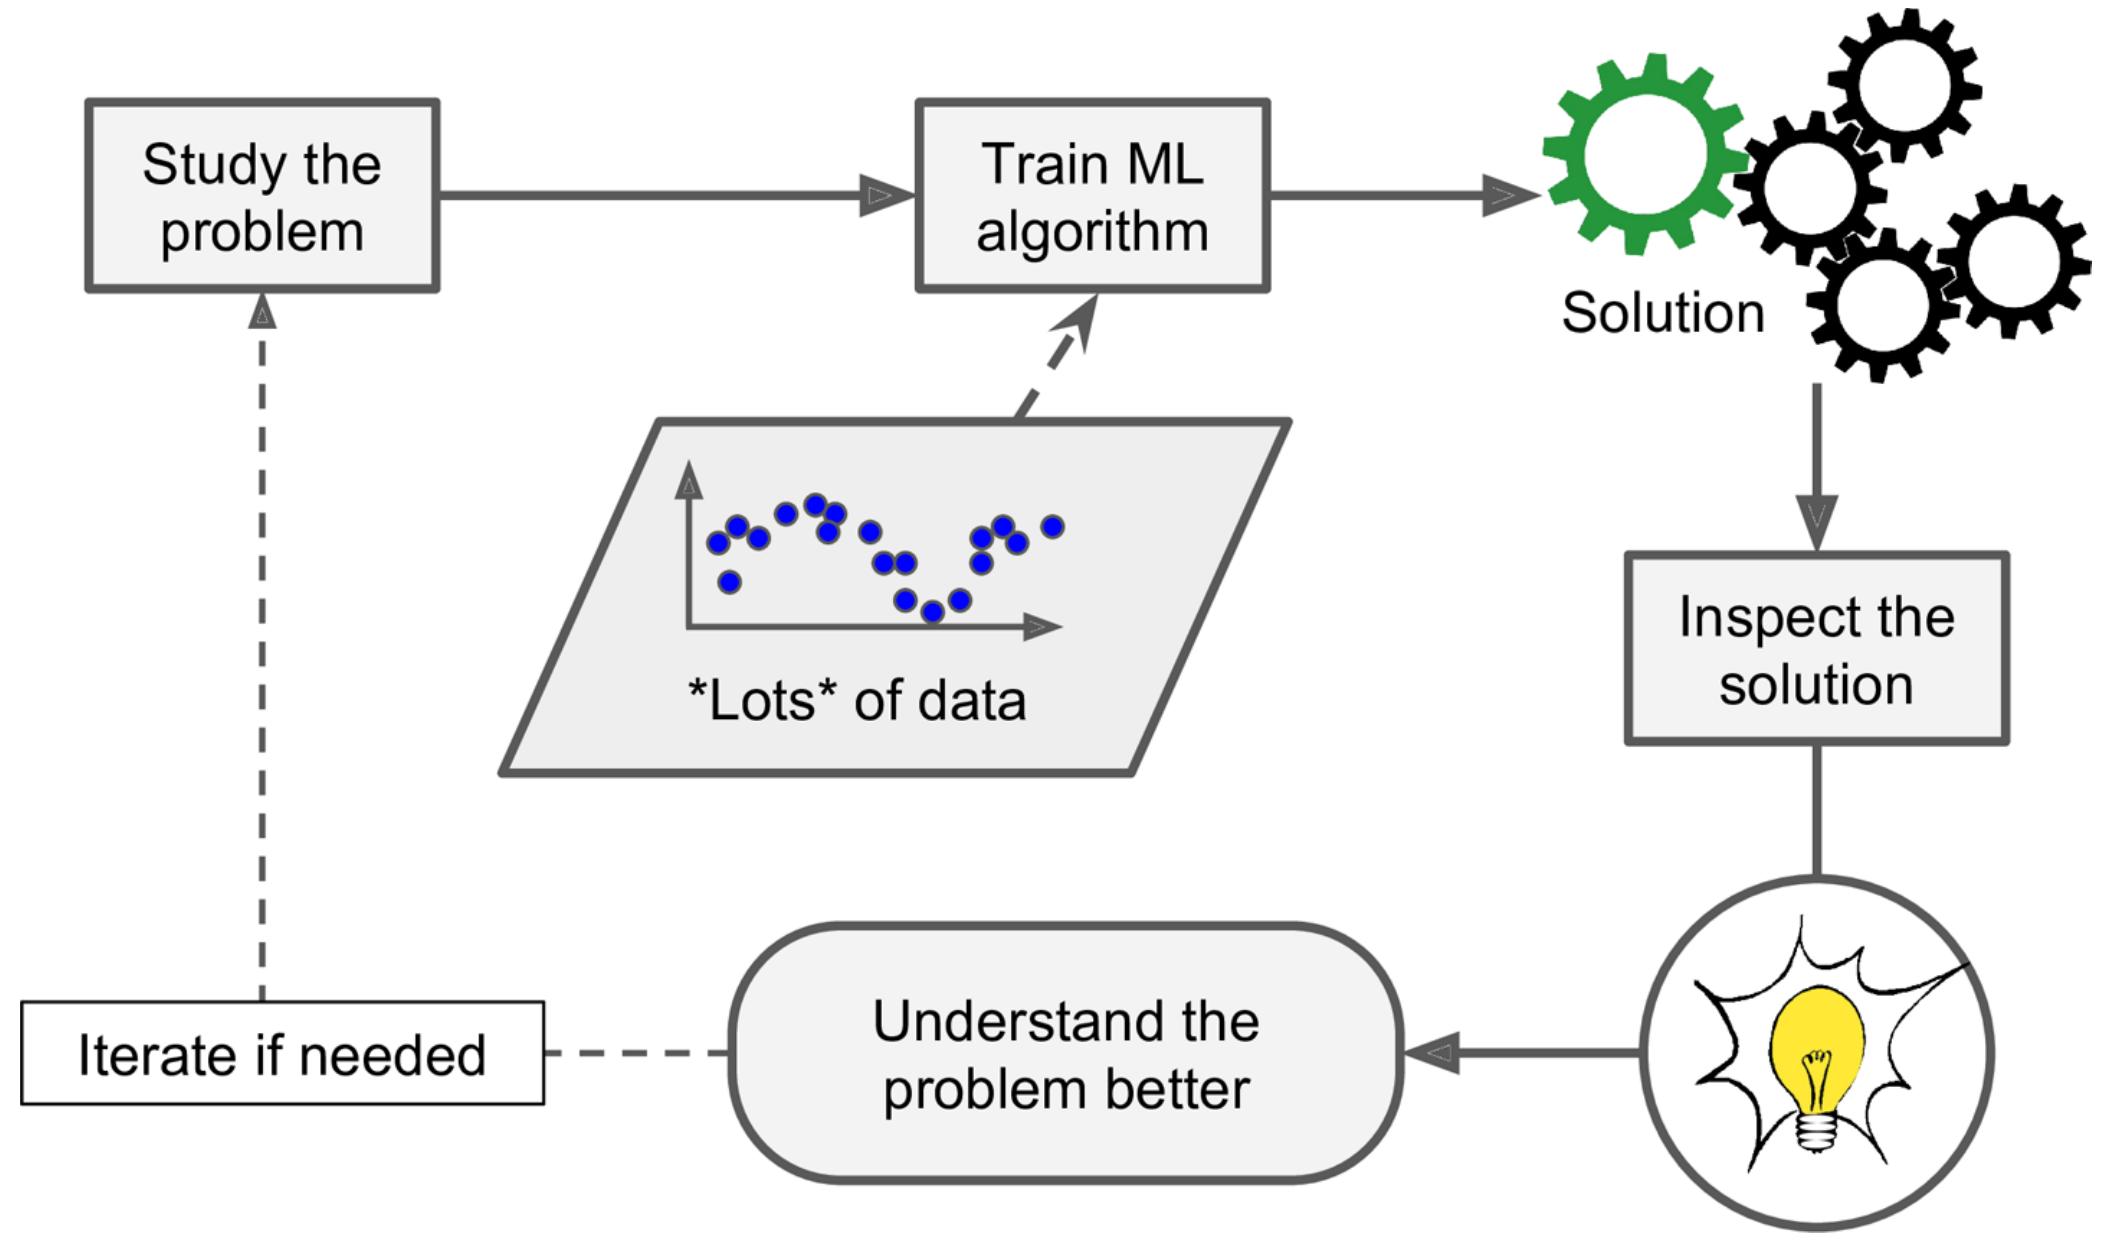
\includegraphics[width=10cm]{ml_workflow}
    \caption{Machine Learning Workflow \parencite{geron2019hands}}%
    \label{fig:workflow}
  \end{figure}
\end{frame}

\begin{frame}{Supervised Learning}
  \begin{figure}[!htbp]
    \centering
    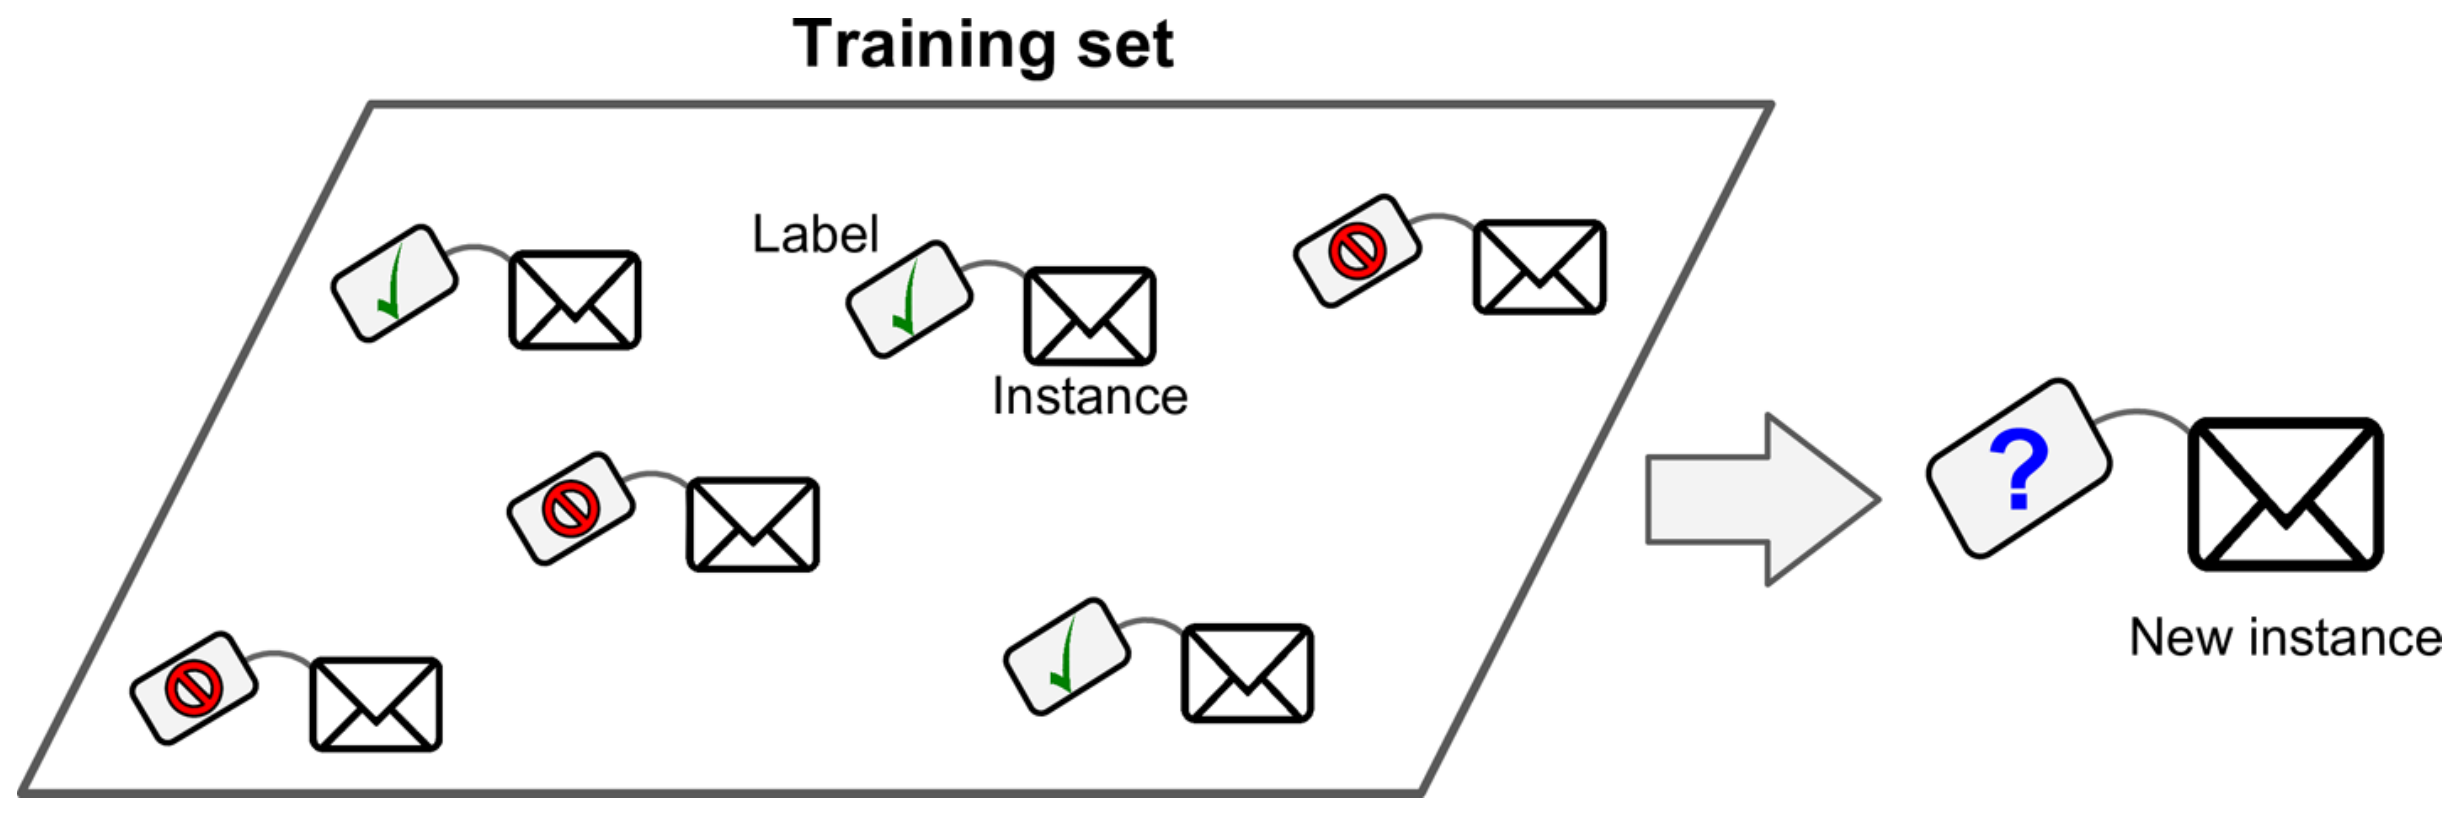
\includegraphics[width=8cm]{data}
    \caption{Struktur der Daten bei Supervised Learning \parencite{geron2019hands}}%
    \label{fig:data}
  \end{figure}

  \only<2->{
    \small
    \begin{block}{Definition Supervised Learning}
      \enquote{In supervised learning, the dataset is the collection of labeled examples
      \({\{(\mathbf{x}_i, y_i)\}}_{i=1}^N\). Each element \(\mathbf{x}_i\) among
      \(N\) is called a feature vector. A feature vector is a vector in which each
      dimension \(j = 1, \ldots , D\) contains a value that describes the example
      somehow [\ldots]. The goal of a supervised learning algorithm is to use the
      dataset to produce a model, that takes a feature vector \(\mathbf{x}\) as
      input and outputs information that allow deducing the label \(\hat{y}\) for
      this feature vector.} \parencite{burkov2019hundred}
    \end{block}
  }
\end{frame}

\begin{frame}{Beispiel: Datensatz für Supervised Learning}
  \begin{minipage}{.6\textwidth}
    \centering
    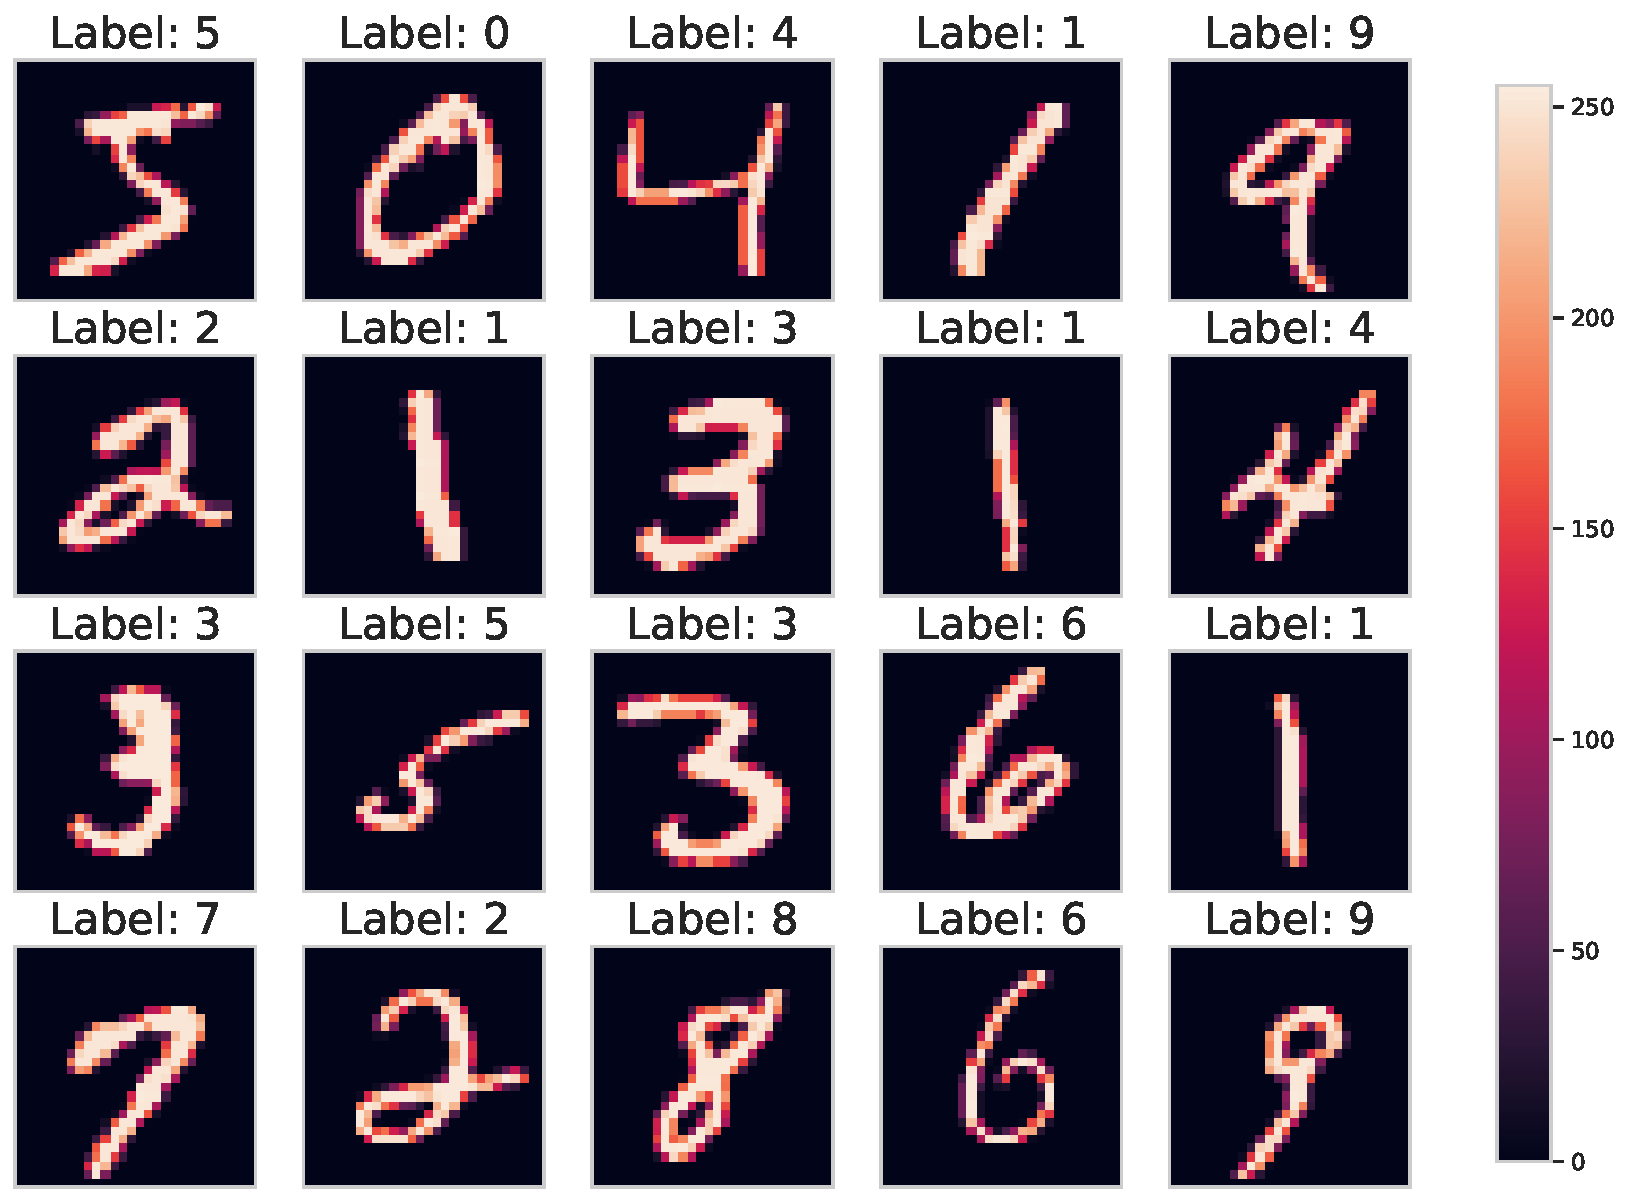
\includegraphics[width=\textwidth]{mnist}
  \end{minipage}\hfill%
  \begin{minipage}{.4\textwidth}
    \begin{itemize}
    \item Insgesamt 70000 Bilder
    \item Bildgröße: 28 \(\times\) 28 Pixel
    \item Abgebildet: Handgeschriebene Ziffern von 0 bis 9
    \item Quelle: Yann LeCun et al \parencite{lecun1998gradient}
    \end{itemize}
  \end{minipage}
\end{frame}

\begin{frame}{Beispiel: Datensatz für Supervised Learning}
  \begin{minipage}{.6\textwidth}
    \centering 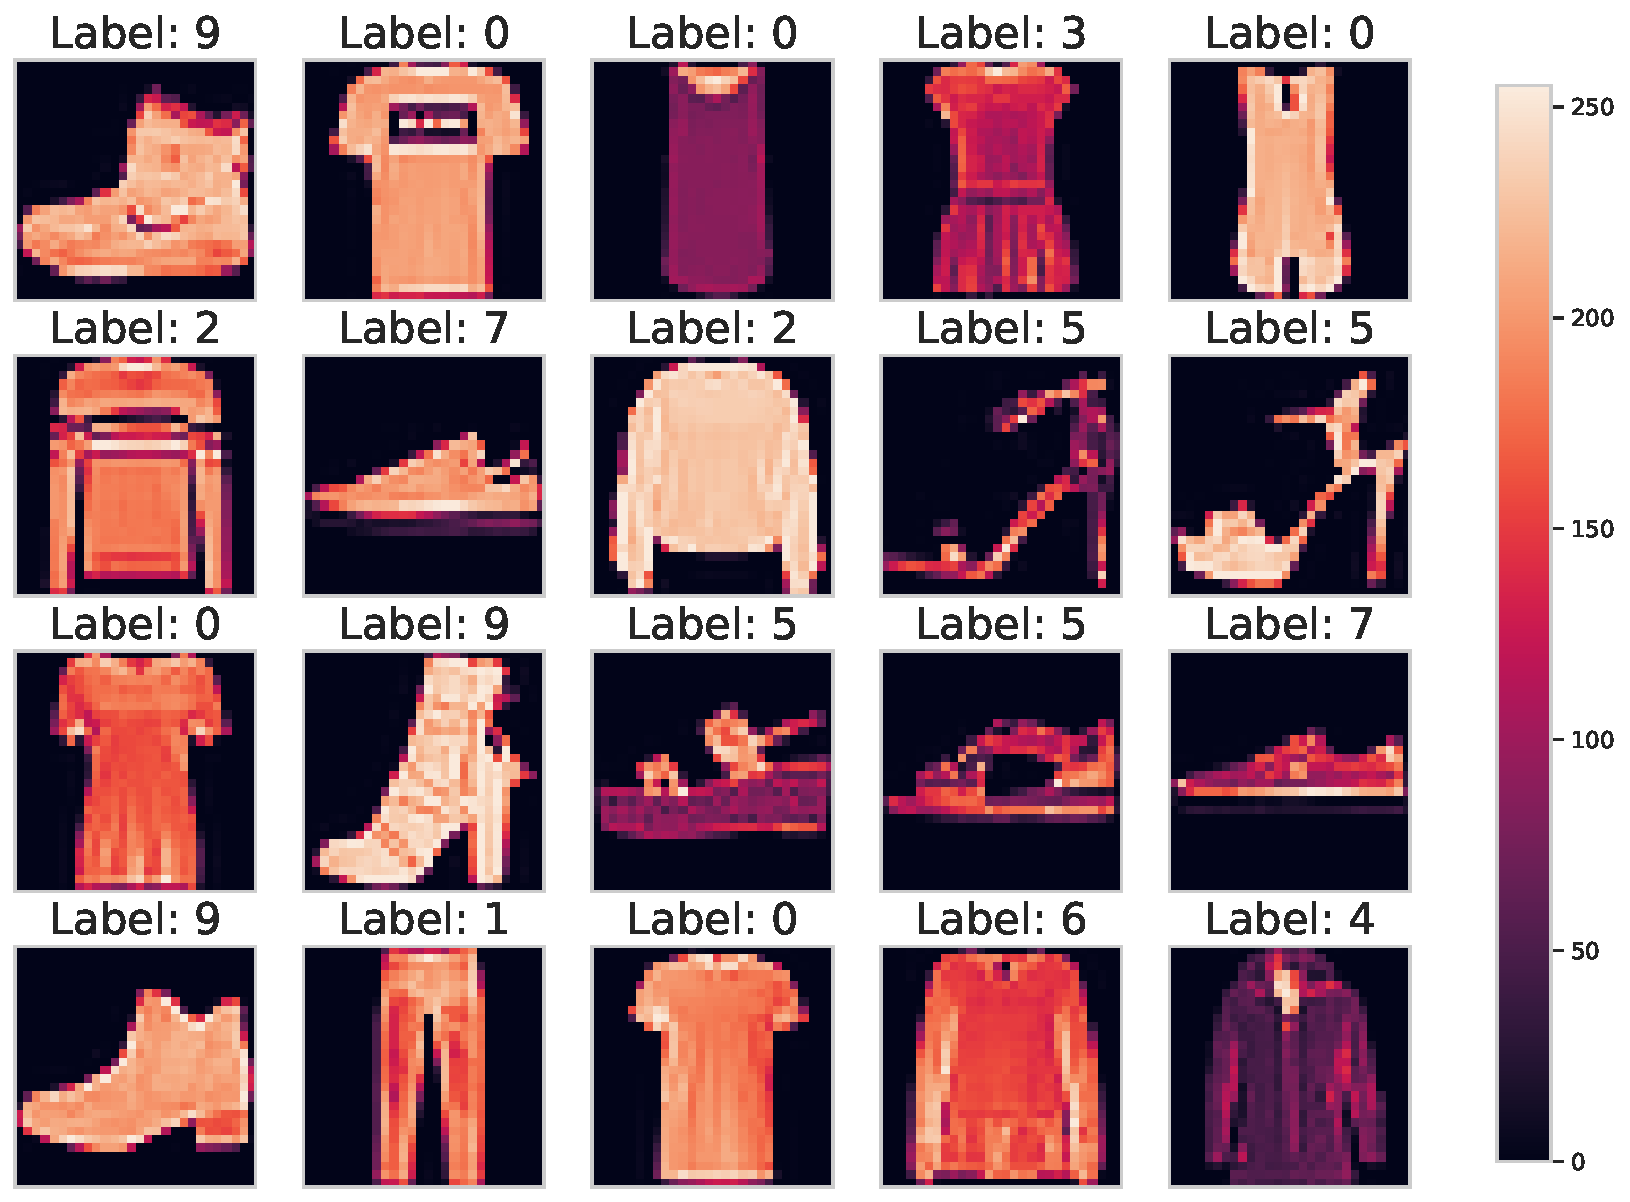
\includegraphics[width=\textwidth]{fashion_mnist}
  \end{minipage}\hfill%
  \begin{minipage}{.4\textwidth}
    \begin{itemize}
    \item Insgesamt 70000 Bilder
    \item Bildgröße: 28 \(\times\) 28 Pixel
    \item Abgebildet: Kleidungsstücke 
    \item Quelle: Zalando Research \parencite{xiao2017fashion}
    \end{itemize}

    \vspace{.5cm}

    \tiny

    \centering
    \begin{tabular}{ll}
      \toprule
      \textbf{Label} & 	\textbf{Description}\\
      \midrule
      0 & 	T-shirt/top\\
      1 & 	Trouser\\
      2 & 	Pullover\\
      3 & 	Dress\\
      4 & 	Coat\\
      5 & 	Sandal\\
      6 & 	Shirt\\
      7 & 	Sneaker\\
      8 & 	Bag\\
      9 & 	Ankle boot\\
      \bottomrule
    \end{tabular}

  \end{minipage}

\end{frame}

%%% Local Variables:
%%% mode: latex
%%% TeX-master: "../präsentation"
%%% End:

\section{Künstliche Neuronale Netze}%
\label{sec:ann}

\begin{frame}{Künstliches Neuron}
  \begin{minipage}{.65\textwidth}
    \begin{tikzpicture}[->, >=stealth, thick, scale=.8]
      \node [circle split,draw,rotate=90] (z) at (0, 0) {\rotatebox{-90}{$\displaystyle\sum$} \nodepart{lower} \rotatebox{-90}{$\sigma(z)$}};
      \foreach \i in {5,...,1} {
        \node (x-\i) at (-7, 4.5+1.5*-\i) {\(x_{\i}\)};
        \path (x-\i) edge node[above] {\(w_{\i}\)} (z);
      }
      \node (y) at (4, 0) {\(a\)};
      \path (z) edge (y);
      \node (b) at (0, 2.5) {\(b\)};
      \draw (b) -- (z);
    \end{tikzpicture}
  \end{minipage}%
  \begin{minipage}{.35\textwidth}
    \uncover<2->{
      \begin{flushright}
        \begin{tabular}{cl}
          \toprule
          \(\mathbf{x}\)  & Inputvektor\\
          \(\mathbf{w}\)  & Gewichtsvektor\\
          \(b\)  & Bias\\
          \(z\)  & Zwischensumme \(\left(\sum\right)\)\\
          \(\sigma(x)\)  & Aktivierungsfunktion\\
          \(a\)  & Aktivierung/ Output\\
          \bottomrule
        \end{tabular}
      \end{flushright}
    }
  \end{minipage}

  \only<3>{
    \[z = \sum_{i}x_{i}w_i + b = \mathbf{xw} + b\]

    {\centering\(\Rightarrow z\) wird für spätere Parameteroptimierung benötigt\par}
  }
\end{frame}

\begin{frame}{Aktivierungsfunktion \(\sigma(x)\)}
  \begin{minipage}{.45\textwidth}
    \(\Rightarrow\) Es gibt eine Vielzahl verschiedener Aktivierungsfunktionen für unterschiedliche Problemstellungen, für uns soll jedoch lediglich die \textbf{Sigmoid-Funktion} relevant sein:

    \vspace{1cm}

    \[\sigma(x) = \frac{1}{1 + e^{-x}}\]
  \end{minipage}\hfill%
  \begin{minipage}{.5\textwidth}
    \only<2>{
      \begin{tikzpicture}
        \begin{axis}[width=\textwidth, mlineplot, samples=50, ymin=-.1, ymax=1.1, domain=-10:10, title=Sigmoid-Funktion, xlabel=\(x\), ylabel=\(\sigma(x)\)]
          \addplot{1/(1+exp(-x))};
        \end{axis}
      \end{tikzpicture}
    }
  \end{minipage}

\end{frame}

\begin{frame}{Architektur eines Neuronalen Netzwerks}
  \def\layersep{3.5cm}
  \begin{center}
    \alt<2>{
      \begin{tikzpicture}[->, >=stealth, node distance=\layersep]
        \tikzstyle{every pin edge}=[<-,shorten <=1pt]
        \tikzstyle{neuron}=[circle,draw,minimum size=17pt,inner sep=0pt]
        
        % Draw the input layer nodes
        \foreach \y in {1,...,3}
        \node[neuron, pin=left:\(x_{\y}\)] (I-\y) at (0,-\y) {};

        % Draw the nodes for the second hidden layer
        \foreach \y in {1,...,5}
        \path[yshift=(5cm - 3cm)/2] node[neuron] (H1-\y) at (\layersep,-\y cm) {};

        % Draw the output layer nodes
        \foreach \y in {1,...,2}
        \path[yshift=(2cm - 3cm)/2] node[neuron,pin={[pin edge={->}]right:\(y_{\y}\)}] (O-\y) at (2*\layersep,-\y cm) {};

        \foreach \source in {1,...,3}
        \foreach \dest in {1,...,5}
        \path (I-\source) edge (H1-\dest);

        \foreach \source in {1,...,5}
        \foreach \dest in {1,...,2}
        \path (H1-\source) edge (O-\dest);

        \node[above of=H1-1, node distance=1cm] (hidden) {Hidden Layer};
        \node[right of=hidden] (output) {Output Layer};
        \node[left of=hidden] (input) {Input Layer};
      }{
        \begin{tikzpicture}[->, >=stealth]
          \tikzstyle{every pin edge}=[<-,shorten <=1pt]
          \tikzstyle{neuron}=[circle,draw,minimum size=17pt,inner sep=0pt]
          
          % Draw the input layer nodes
          \foreach \y in {1,...,3}
          \node[neuron, pin=left:] (I-\y) at (0,-\y) {};

          % Draw the nodes for the second hidden layer
          \foreach \y in {1,...,5}
          \path[yshift=(5cm - 3cm)/2] node[neuron] (H1-\y) at (\layersep,-\y cm) {};

          % Draw the output layer nodes
          \foreach \y in {1,...,2}
          \path[yshift=(2cm - 3cm)/2] node[neuron,pin={[pin edge={->}]right:}] (O-\y) at (2*\layersep,-\y cm) {};

          \foreach \source in {1,...,3}
          \foreach \dest in {1,...,5}
          \path (I-\source) edge (H1-\dest);

          \foreach \source in {1,...,5}
          \foreach \dest in {1,...,2}
          \path (H1-\source) edge (O-\dest);
        }
      \end{tikzpicture}
    \end{center}
  \end{frame}

  \begin{frame}{Deep Neural Network}
    \begin{center}
      \dnn{5, 6, 5, 7, 3}
    \end{center}
  \end{frame}

  \begin{frame}{Target-Architektur zur Klassifikation von MNIST}
    \def\layersep{2.5cm}
    \begin{center}
      \begin{tikzpicture}[->, >=stealth, node distance=\layersep]
        \tikzstyle{every pin edge}=[<-,shorten <=1pt]
        \tikzstyle{neuron}=[circle,draw,minimum size=17pt,inner sep=0pt]
        
        \node[neuron, pin=left:\(x_{1}\)] (I-1) at (0,-1) {}; \node[neuron,
        pin=left:\(x_{2}\)] (I-2) at (0,-2) {}; \node[neuron,
        pin=left:\(x_{3}\)] (I-3) at (0,-3) {}; \node at (0, -4) {\(\vdots\)};
        \node[neuron, pin=left:\(x_{784}\)] (I-4) at (0,-5) {};

        \path[yshift=(6cm - 5cm)/2] node[neuron] (H1-1) at (\layersep,-1 cm) {};
        \path[yshift=(6cm - 5cm)/2] node[neuron] (H1-2) at (\layersep,-2 cm) {};
        \path[yshift=(6cm - 5cm)/2] node[neuron] (H1-3) at (\layersep,-3 cm) {};
        \path[yshift=(6cm - 5cm)/2] node[neuron] (H1-4) at (\layersep,-4 cm) {};
        \path[yshift=(6cm - 5cm)/2] node at (\layersep, -4.7cm) {$\vdots$};
        \path[yshift=(6cm - 5cm)/2] node[neuron] (H1-5) at (\layersep,-6 cm) {};

        \path node[neuron] (H2-1) at (2*\layersep,-1 cm) {}; \path node[neuron]
        (H2-2) at (2*\layersep,-2 cm) {}; \path node[neuron] (H2-3) at
        (2*\layersep,-3 cm) {}; \path node at (2*\layersep, -3.7cm) {$\vdots$};
        \path node[neuron] (H2-4) at (2*\layersep,-5 cm) {};

        \path[yshift=(2cm - 3cm)/2] node[neuron,pin={[pin
          edge={->}]right:\(y_{1}\)}] (O-1) at (3*\layersep,-1 cm) {};
        \path[yshift=(2cm - 3cm)/2] node[neuron,pin={[pin
          edge={->}]right:\(y_{2}\)}] (O-2) at (3*\layersep,-2 cm) {};
        \path[yshift=(2cm - 3cm)/2] node at (3*\layersep, -3cm) {$\vdots$};
        \path[yshift=(2cm - 3cm)/2] node[neuron,pin={[pin
          edge={->}]right:\(y_{10}\)}] (O-3) at (3*\layersep,-4 cm) {};

        \foreach \source in {1,...,4} \foreach \dest in {1,...,5} \path
        (I-\source) edge (H1-\dest);

        \foreach \source in {1,...,5} \foreach \dest in {1,...,4} \path
        (H1-\source) edge (H2-\dest);

        \foreach \source in {1,...,4} \foreach \dest in {1,...,3} \path
        (H2-\source) edge (O-\dest);

        \foreach \y [count=\i] in {1,2,3,4,30} \node[node distance=14pt, above
        of=H1-\i] {\tiny\(H^1_{\y}\)};

        \foreach \y [count=\i] in {1,2,3,15} \node[node distance=14pt, above
        of=H2-\i] {\tiny\(H^2_{\y}\)};
      \end{tikzpicture}
    \end{center}
  \end{frame}
  
  \begin{frame}{Vektorisierung der Gewichte \(w\) und der Biases \(b\)}
    \def\layersep{2.5cm}
    \begin{tikzpicture}[->, >=stealth, node distance=\layersep, spy using outlines={circle, magnification=5, size=7cm, connect spies}]
      \begin{scope}[scale=.5, transform shape]
        \tikzstyle{every pin edge}=[<-,shorten <=1pt]
        \tikzstyle{neuron}=[circle,draw,minimum size=17pt,inner sep=0pt]

        % Input Neurons
        \node[neuron, pin=left:\(x_{1}\)] (I-1) at (0,-1) {};
        \node[neuron, pin=left:\(x_{2}\)] (I-2) at (0,-2) {};
        \node[neuron, pin=left:\(x_{3}\)] (I-3) at (0,-3) {};
        \node at (0, -4) {\(\vdots\)};
        \node[neuron, pin=left:\(x_{784}\)] (I-4) at (0,-5) {};

        % Neurons in first hidden layer
        \path[yshift=(6cm - 5cm)/2] node[neuron] (H1-1) at (\layersep,-1 cm) {};
        \path[yshift=(6cm - 5cm)/2] node[neuron] (H1-2) at (\layersep,-2 cm) {};
        \path[yshift=(6cm - 5cm)/2] node[neuron] (H1-3) at (\layersep,-3 cm) {};
        \path[yshift=(6cm - 5cm)/2] node[neuron] (H1-4) at (\layersep,-4 cm) {};
        \path[yshift=(6cm - 5cm)/2] node at (\layersep, -4.7cm) {$\vdots$};
        \path[yshift=(6cm - 5cm)/2] node[neuron] (H1-5) at (\layersep,-6 cm) {};

        % Neurons in second hidden layer
        \path node[neuron] (H2-1) at (2*\layersep,-1 cm) {};
        \path node[neuron] (H2-2) at (2*\layersep,-2 cm) {};
        \path node[neuron] (H2-3) at (2*\layersep,-3 cm) {};
        \path node at (2*\layersep, -3.7cm) {$\vdots$};
        \path node[neuron] (H2-4) at (2*\layersep,-5 cm) {};

        % Neurons in output layer
        \path[yshift=(2cm - 3cm)/2] node[neuron,pin={[pin edge={->}]right:\(y_{1}\)}] (O-1) at (3*\layersep,-1 cm) {};
        \path[yshift=(2cm - 3cm)/2] node[neuron,pin={[pin edge={->}]right:\(y_{2}\)}] (O-2) at (3*\layersep,-2 cm) {};
        \path[yshift=(2cm - 3cm)/2] node at (3*\layersep, -3cm) {$\vdots$};
        \path[yshift=(2cm - 3cm)/2] node[neuron,pin={[pin edge={->}]right:\(y_{10}\)}] (O-3) at (3*\layersep,-4 cm) {};

        \foreach \source in {1,...,4}
        \foreach \dest in {1,...,5}
        \path (I-\source) edge (H1-\dest);

        \foreach \source in {1,...,5}
        \foreach \dest in {1,...,4}
        \path (H1-\source) edge (H2-\dest);

        \foreach \source in {1,...,4}
        \foreach \dest in {1,...,3}
        \path (H2-\source) edge (O-\dest);

        \foreach \y [count=\i] in {1,2,3,4,30}
        \node[node distance=14pt, above of=H1-\i] {\tiny\(H^1_{\y}\)};

        \foreach \y [count=\i] in {1,2,3,15}
        \node[node distance=14pt, above of=H2-\i] {\tiny\(H^2_{\y}\)};

        \spy[myblue] on (H1-1) in node (a) at (10, -3.5);
      \end{scope}
      \only<2->{
        \begin{scope}[myorange, yshift=-1.5cm]
          \draw[-, line width=.7mm, black] (10, -1.25cm) -- (10, -2.75cm);
          \node (sum) at (9.65, -2) {\large\(\sum\)};
          \node (act) at (10.4, -2) {\(\sigma(z)\)};
          \node (x1) at (7.8, -2.1) {\small\(x_1w^1_{1,1}\)};
          \node (x2) at (7.6, -3) {\small\(x_2w^1_{1,2}\)};
          \node (x3) at (7.8, -3.65) {\small\(x_3w^1_{1,3}\)};
          \node[fill=white] (x4) at (9, -3.8) {\small\(x_{784}w^1_{1,784}\)};
          \node (a1) at (12, -2.15) {\small\(a^1_1\)};
          \node (a2) at (11.8, -2.8) {\small\(a^1_1\)};
          \node (a3) at (11.6, -3.3) {\small\(a^1_1\)};
          \node (a4) at (11.05, -3.4) {\small\(a^1_1\)};
        \end{scope}
      }
      \uncover<3->{
        \node at (2.5, -5) {\footnotesize\(\displaystyle \mathbf{W^2} =
          \begin{bmatrix}
            w^2_{1,1} & w^2_{2,1} & \cdots & w^2_{30,1}\\[1em]
            w^2_{1,2} & w^2_{2,2} & \cdots & w^2_{30,2}\\[1em]
            \vdots & \vdots & \ddots & \vdots\\[1em]
            w^2_{1,784} & w^2_{2,784} & \cdots & w^2_{30,784}
          \end{bmatrix};~
          \mathbf{b^2} =
          \begin{bmatrix}
            b^2_1\\[1em]
            b^2_2\\[1em]
            \vdots\\[1em]
            b^2_{30}
          \end{bmatrix}
          \)};
      }
    \end{tikzpicture}
  \end{frame}

  \begin{frame}{Output eines neuronalen Netzwerks berechnen}
    Gegeben:
    \begin{itemize}
    \item Inputvektor \(\mathbf{x}\)
    \item Gewichtsmatrizen \(\mathbf{W}^{2 \ldots 4}\)
    \item Biasvektoren \(\mathbf{b}^{2 \ldots 4}\)
    \end{itemize}

    \begin{align*}
      \mathbf{a^{1}} &= \mathbf{x}\\
      \mathbf{a^{2}} &= \sigma(\mathbf{W^{2}a^{1}} + \mathbf{b^{2}})\\
      \mathbf{a^{3}} &= \sigma(\mathbf{W^{3}a^{2}} + \mathbf{b^{3}})\\
      \mathbf{a^{4}} &= \sigma(\mathbf{W^{4}a^{3}} + \mathbf{b^{4}}) = \mathbf{\hat{y}}
    \end{align*}
  \end{frame}

  %%% Local Variables:
  %%% mode: latex
  %%% TeX-master: "../präsentation"
  %%% End:

\section{Training}%
\label{sec:train}

\subsection{Loss-Funktion}%
\label{sec:loss}

\begin{frame}{Loss-Funktion}
  \begin{itemize}
  \item Dient zur Berechnung des Fehlers während dem Training
  \item Trainingsfehler soll minimiert werden
  \item \(\Rightarrow\) wir suchen den Punkt, an dem die Ableitung der
    Loss-Funktion \(0\) wird, der Fehler also nicht mehr abnimmt
  \item Es gibt eine Vielzahl an Loss-Funktionen, wir betrachten hier
    die \enquote{\textbf{Mean Squared Error (MSE)}}:
  \end{itemize}

  \vspace{.6cm}

  \begin{minipage}{.4\linewidth}
    \[C(w, b) = \frac{1}{2m} \sum_{x=1}^{m} (y(x) - \hat{y}(x))^2\]
  \end{minipage}\hfill%
  \begin{minipage}{.55\linewidth}
    \uncover<2->{
      \begin{tabular}{ll}
        \toprule
        \(C(w, b)\) & Cost in Abhängigkeit von \(w\) und \(b\)\\
        \(m\) & Anzahl der Trainingsinstanzen\\
        \(y(x)\) & Gewünschter Output wenn \(x\) Input ist\\
        \(\hat{y}(x)\) & Tatsächlicher Output des Netzwerkes\\
        \bottomrule
      \end{tabular}
    }
  \end{minipage}
\end{frame}

\subsection{Gradient Descent}%
\label{sec:graddesc}

\begin{frame}{Gradient Descent}
  \begin{itemize}
  \item Methode um die Weights \(w\) und Biases \(b\) zu optimieren
  \item Vorgehen: \pause
    \begin{enumerate}
    \item Finde die Änderungsrate des Fehlers in Abhängigkeit von den Weights und Biases (\(\partial C / \partial w; \partial C / \partial b\))\pause
    \item Multipliziere die Änderungsrate mit der Lernrate \(\eta\)\pause
    \item Ziehe das Produkt aus Änderungsrate und Lernrate von den aktuellen Parametern ab\pause
    \item Aktualisiere die alten Parameter durch das Ergebnis des letzten Schrittes
    \end{enumerate}
  \end{itemize}

  \begin{align*}
    w_{k+1} &= w_{k} - \eta \frac{\partial C}{\partial w_{k}}\\[1em]
    b_{k+1} &= b_{k} - \eta \frac{\partial C}{\partial b_{k}}\\
  \end{align*}

\end{frame}

\subsection{Backpropagation}%
\label{sec:backprop}

\begin{frame}{Backpropagation}
    \begin{alertblock}{Problem}
      Wie finde ich die Änderungsraten \(\frac{\partial C}{\partial w}; \frac{\partial C}{\partial b}\), die ich für Gradient Descent benötige?
    \end{alertblock}

\uncover<2->{\(\Rightarrow\) Idee: Divide and conquer; Problem in kleinere, handhabbare Probleme zerlegen}

  \begin{align*}
    \uncover<3->{f(a, b, c, d) &= {({(a + b)} \cdot (c + d))}^{2}\\}
    \uncover<4->{g(a, b) &= a + b\\}
    \uncover<5->{h(c, d) &= c + d\\}
    \uncover<6->{i(g, h) &= g \cdot h\\}
    \uncover<7->{f(i) &= i^{2}}
  \end{align*}
\end{frame}

\begin{frame}{Backpropagation}
  \begin{columns}
    \begin{column}{.4\textwidth}
      \begin{align*}
        f(a, b, c, d) &= {({(a + b)} \cdot (c + d))}^{2}\\
        g(a, b) &= a + b\\
        h(c, d) &= c + d\\
        i(g, h) &= g \cdot h\\
        f(i) &= i^{2}
      \end{align*}
    \end{column}
    \begin{column}{.6\textwidth}
      \begin{tikzpicture}[every node/.style={circle, minimum width=.8cm}]
        \node (a) at (0, 7) {\(a\)};
        \node (b) at (0, 5) {\(b\)};
        \node (c) at (0, 3) {\(c\)};
        \node (d) at (0, 1) {\(d\)};
        \node[draw] (g) at (2, 6) {\(+\)};
        \node[draw] (h) at (2, 2) {\(+\)};
        \node[draw] (i) at (4, 4) {\(\cdot\)};
        \node[draw] (j) at (6, 4) {\(()^{2}\)};
        \draw (a) -- (g);
        \draw (b) -- (g);
        \draw (c) -- (h);
        \draw (d) -- (h);
        \draw (g) -- (i) node[midway, above] {\(g\)};
        \draw (h) -- (i) node[midway, above] {\(h\)};
        \draw (i) -- (j) node[midway, above] {\(i\)};
        \draw (j) -- (7, 4) node[midway, above] {\(f(i)\)};
      \end{tikzpicture}
    \end{column}
  \end{columns}
\end{frame}

\begin{frame}{Backpropagation}

  \vspace{-.2cm}

  \begin{center}
    \begin{tikzpicture}[every node/.style={circle, minimum width=.8cm}]
      \node (a) at (0, 6) {\(a\)};
      \node (b) at (0, 4) {\(b\)};
      \node (c) at (0, 3) {\(c\)};
      \node (d) at (0, 1) {\(d\)};
      \node[draw] (g) at (4, 5) {\(+\)};
      \node[draw] (h) at (4, 2) {\(+\)};
      \node[draw] (i) at (6, 3.5) {\(\cdot\)};
      \node[draw] (j) at (9, 3.5) {\(()^{2}\)};
      \draw (a) -- (g) node[midway,above]{\(\frac{\partial g}{\partial a}\)};
      \draw (b) -- (g);
      \draw (c) -- (h);
      \draw (d) -- (h);
      \draw (g) -- (i) node[midway, above] {\(g\)} node[midway, below] {\(\frac{\partial gh}{\partial g}\)};
      \draw (h) -- (i);
      \draw (i) -- (j) node[midway, above] {\(i\)} node[midway, below]{\(\frac{\partial i}{\partial gh}\)};
      \draw (j) -- (11, 3.5) node[midway, above] {\(f(i)\)} node[midway, below]{\(\frac{\partial f}{\partial i}\)};
    \end{tikzpicture}
  \end{center}

  \vspace{-.4cm}

  \begin{alertblock}{Frage: \(\frac{\partial f}{\partial a}\)?}
    \uncover<2->{\[\frac{\partial f}{\partial a} = \frac{\partial f}{\partial i} \cdot \frac{\partial i}{\partial gh} \cdot \frac{\partial gh}{\partial g} \cdot \frac{\partial g}{\partial a}\]}
  \end{alertblock}
\end{frame}

\subsection{Umsetzung in Keras}

\begin{frame}{Zuvor beschriebene Architektur}
  Pass
\end{frame}

\begin{frame}{Optimierte Architektur}
  \begin{itemize}
  \item Vorteil: Schnellere Konvergenz
  \item Verwendung von optimierter Cost-, Activation- und Gradient-Descent-Funktion
  \end{itemize}
\end{frame}

%%% Local Variables:
%%% mode: latex
%%% TeX-master: "../präsentation"
%%% End:

\section{Umsetzung in Keras}

\begin{frame}[fragile]{Zuvor beschriebene Architektur}
  \begin{lstlisting}
    from tensorflow import keras
    ...
    model = keras.models.Sequential([
      keras.layers.Flatten(input_shape=(28, 28)),
      keras.layers.Dense(30, activation='sigmoid'),
      keras.layers.Dense(15, activation='sigmoid'),
      keras.layers.Dense(10, activation='sigmoid'),
    ])

    model.compile(loss='mse',
                  optimizer=keras.optimizers.SGD(learning_rate=.8),
                  metrics=['accuracy'])

    history = model.fit(X_train, y_train_cat, epochs=10,
                        validation_data=(X_valid, y_valid_cat))
  \end{lstlisting}
\end{frame}

\begin{frame}{Verlauf während des Trainings}
  \begin{center}
    \begin{tikzpicture}
      \begin{axis}[mlineplot,legend style={
          cells={anchor=east},
          legend pos=outer north east,
        }, ymin=0, ymax=1.1, xmin=0.8, xmax=10.2, xlabel=Epoch]
        \addplot table [x=history, y=loss, col sep=comma] {history1.csv};
        \addlegendentry{Loss}
        \addplot table [x=history, y=accuracy, col sep=comma] {history1.csv};
        \addlegendentry{Accuracy}
      \end{axis}
    \end{tikzpicture}
  \end{center}
\end{frame}

\begin{frame}[fragile]{Optimierte Architektur}
  \begin{itemize}
  \item Vorteil: Schnellere Konvergenz
  \item Verwendung von optimierter Cost-, Activation- und Gradient-Descent-Funktion
  \end{itemize}
  \begin{lstlisting}
    model = keras.models.Sequential([
      keras.layers.Flatten(input_shape=(28, 28)),
      keras.layers.Dense(30, activation='relu'),
      keras.layers.Dense(15, activation='relu'),
      keras.layers.Dense(10, activation='softmax'),
    ])

    model.compile(loss='sparse_categorical_crossentropy',
                  optimizer='Adam',
                  metrics=['accuracy'])
  \end{lstlisting}
\end{frame}

\begin{frame}{Verlauf während des Trainings}
  \begin{center}
    \begin{tikzpicture}
      \begin{axis}[mlineplot,legend style={
          cells={anchor=east},
          legend pos=outer north east,
        }, ymin=0, ymax=1.1, xmin=0.8, xmax=10.2, xlabel=Epoch]
        \addplot table [x=history, y=loss, col sep=comma] {history2.csv};
        \addlegendentry{Loss}
        \addplot table [x=history, y=accuracy, col sep=comma] {history2.csv};
        \addlegendentry{Accuracy}
      \end{axis}
    \end{tikzpicture}
  \end{center}
\end{frame}


%%% Local Variables:
%%% mode: latex
%%% TeX-master: "../präsentation"
%%% End:


\begin{frame}[standout]
  Fragen?
\end{frame}

\printbibliography[title=Literaturverzeichnis]

\end{document}